\section{Conference Management}

% ===============================================
% This is the hierarchy breakdown
% ===============================================
\begin{center}
	\begin{tikzpicture}[
		chair/.style={rectangle, text centered, draw,fill=blue!20, execute at begin node={\begin{varwidth}{9em}},
   		execute at end node={\end{varwidth}}},
   		committee/.style={rectangle,draw,fill=green!40, text centered, execute at begin node={\begin{varwidth}{7em}},
   		execute at end node={\end{varwidth}}},
   		coordinator/.style={rectangle,draw,fill=red!30, text centered, execute at begin node={\begin{varwidth}{7em}},
   		execute at end node={\end{varwidth}}},
		grandchild/.style={grow=down,xshift=1em,anchor=west,
		edge from parent path={(\tikzparentnode.south) |- (\tikzchildnode.west)}, execute at begin node={\begin{varwidth}{8em}},
   		execute at end node={\end{varwidth}}},
		first/.style={level distance=12ex},
		second/.style={level distance=24ex},
		third/.style={level distance=36ex},
		level 1/.style={sibling distance=11em}]
	    % Parents
	    \coordinate
	      child[grow=left] {node[chair,anchor=east]{General Co-Chair \\ (Sam Dotson)}}
	      child[grow=right] {node[chair,anchor=west]{Technical Co-Chair\\ (Jeremy Mettler)}}
	      child[grow=down,level distance=3ex]
	    [edge from parent fork down]
	    % Children and grandchildren
	    child{node[committee] {Non-Technical Subcommittee}
	      child[grandchild,first] {node[chair]{Logistics Chair}}
	      child[grandchild,second] {node[coordinator]{Hotels and Transportation}}
	      child[grandchild,third] {node[coordinator] {Hospitality and Catering}}}
	    child {node[committee] {Communications Subcommittee}
	      child[grandchild, first] {node[chair] {Publications Chair}}
	      child[grandchild, second] {node[coordinator]{Media}}
	      child[grandchild, third] {node[coordinator] {Program}}}
	    child{node[committee] {Financial Subcommittee}
	      child[grandchild,first] {node[chair]{Financial Chair}}
	      child[grandchild,second] {node[coordinator]{Registration}}
	      child[grandchild,third] {node[coordinator]{Sponsorship}}}
	    child {node[committee]{Technical Subcommittee}
	      child[grandchild,first] {node[chair]{Sessions Chair}}
	      child[grandchild,second] {node[coordinator]{Workshops}}
	      child[grandchild,third] {node[coordinator]{Career Fair}}};
	\end{tikzpicture}
\end{center}
% ===============================================
% ===============================================
% ===============================================


\subsection{Position Responsibilities}
The three co-chairs are responsible for setting up major milestones and 
ensuring that those milestones are met. Together they oversee all three subcommittees but 
are each primarily in charge of one. They will serve as the primary contacts between subcommittee
chairs and the faculty as well as professionals. The co-chairs have the final word on all 
conference decisions. They serve as the face of the conference and 

\begin{itemize}
	\item $\large\textbf{\textit{General Co-Chair}}$\\
	In addition to the responsibilities outlined above, the General Co-Chair primarily oversees the
	Non-technical Subcommittee and the Media Coordinator. He works with the Technical Co-Chair to plan full committee
	meetings and completes any remaining tasks to ensure that milestones are met.
	\item $\large\textbf{\textit{Technical Co-Chair}}$\\
	In addition to the responsibilities outlined above, the Technical Co-Chair primarily oversees the
	Technical Subcommittee. Works with the General Co-Chair to plan full committee meetings and completes any remaining tasks to ensure that milestones are met.
	\item $\large\textbf{\textit{Financial Co-Chair}}$\\
	In addition to the responsibilities outlined above, the Financial Co-Chair primarily oversees the Financial Subcommittee. The Financial Co-Chair is also responsible for interacting with businesses, the university, and ANS National for sponsorship needs. He completes any remaining tasks to ensure that milestones are met.

	\item $\textbf{Non-Technical Subcommittee}$\\
	The Non-Technical Subcommittee oversees, arranges, and executes all actions related to hospitality, transportation, special events, and non-technical workshops and panels. This committee keeps the theme of the conference in mind when organizing all events. They ensure that the conference runs smoothly.
	\begin{itemize}
		\item[$\circ$] $\textbf{Logistics Chair}$\\
		The Logistics Chair is in charge of planning all tours and non-technical workshops and panels. Organizes speakers during dinners. Recruits student volunteers to staff events and sessions during the conference.
		Also responsible for keeping track of the subcommittee and reporting to the Co-Chairs.
		\item[$\circ$] $\textbf{Hotels and Transportation Coordinator}$\\
		Coordinates with ANS National to negotiate room rates and room blocks for hotels. Reserves busses for the 
		necessary times and events. Works with the Hospitality and Catering Coordinator and the Logistics Chair.
		\item[$\circ$] $\textbf{Hospitality and Catering Coordinator}$\\
		Responsible for planning and organizing all catered meals for the conference. that includes contacting the catering services, reserving the venues where meals are held, and making sure the venues are staffed.
		\item[$\circ$]$\textbf{Tours Coordinator}$\\
		The tours coordinator organizes tours and works with the transportation coordinator to ensure that transportation is available during the conference for these tours.
		\item[$\circ$]$\textbf{Program Coordinator}$\\
		The program coordinator creates programs for the conference, sets the conference schedule to minimize overlap between events and increase student involvement. Communicates with other coordinators and subcommittees about the schedule of events. Designs and purchases T-shirts for attendees. Arranges gift bags for attendees. Works with sponsorship coordinator to create gift bags.
	\end{itemize}
	\item $\textbf{Financial Subcommittee}$\\
	The Financial Subcommittee oversees, arranges, and executes all actions related to banking, sponsorship, registration, reimbursement, budgeting, and monetary exchanges. This committee works closely with the General and Technical Co-Chairs.
	\begin{itemize}
		\item[$\circ$] $\textbf{Account Coordinator}$\\
		Manages the ANS Planning Committee account with Busey Bank and ANS National. The account coordinator is also responsible for keeping track of receipts, setting a budget for the committee, keeps track of all transactions, 
		\item[$\circ$] $\textbf{Registration Coordinator }$
		Handles the registration for professional and student attendees. Communicates the number of attendees to the Program Coordinator. 
		\item[$\circ$] $\textbf{Sponsorship Coordinator}$\\
		Assists the Financial Co-Chair with matters involving sponsorship as well as working closely with the Registration and Account Coordinators and the General and Technical Co-Chairs. Works with the Program Coordinator on gift bag items and works with the Career Fair Coordinator.
	\end{itemize}
	\item $\textbf{Technical Subcommittee}$\\
	The Technical Subcommittee works with the Technical Co-Chair to process student abstracts and set up 
	technical workshops, panels and sessions. 
	\begin{itemize}
		\item[$\circ$] $\textbf{Technical Subcommittee Chair}$\\
		 Also responsible for ensuring that judges understand the judging criteria, and organizes the award ceremony.
		Keeps track of subcommittee progress and reports to the General and Technical Co-chairs.
		\item[$\circ$] $\textbf{Sessions Coordinator}$\\
		Responsible for organizing presentation, poster sessions, and technical
		panels. Makes sure that all rooms are properly set up with equipment to ensure smooth technical sessions.
		\item[$\circ$] $\textbf{Workshops Coordinator}$\\
		Organizes workshops locations, times, staffing, costs, supplies, student enrollment
		and any other tasks required to have successful workshops. Also assists the Sessions Chair when needed.
		\item[$\circ$] $\textbf{Career Fair Coordinator}$\\
		Oversees staffing and support for the career fair as well as working with the Sponsorship
		Coordinator to ensure a successful career fair. Also assists the Sessions Chair when needed.
	\end{itemize}
	\item $\textbf{Media Coordinator}$\\
		The Media Coordinator is reponsible for designing the conference website, constantly updating social media presence,
		and obtains information from other members of the planning committee for the website. 
\end{itemize}

\newpage
\subsection{Planning Committee Biographies}

\setlength\intextsep{0pt}
\begin{wrapfigure}{L}{0.35\textwidth}
	\begin{center}
		\vspace{-\baselineskip}
		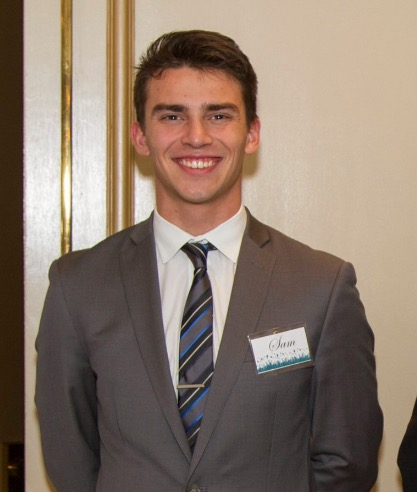
\includegraphics[height=15\baselineskip]{dotsons2.jpg}
	\end{center}
\end{wrapfigure}
$\textbf{General Co-Chair - Sam Dotson}$\\
Sam graduated with a B.S. in Physics from UIUC in 2019. He attended his first ANS student conference in April 2019 and was so inspired by his experience that he decided to pursue graduate work in nuclear engineering rather than physics. Now he does research on machine learning applications and computational reactor physics with Dr. Kathryn Huff in the ARFC group. Hosting a student conference that will inspire others the way he was inspired is one of his top priorities this year. He has experience planning activities for student organizations such as Guidance for Physics Students (GPS) and has experience fundraising for the College of Lake County (CLC). He helped set a record amount of donations at the 2016 CLC Foundation Gala, where he was an invited speaker and volunteer. He will be attending the ANS National conference in November 2019, as well as the ANS Student Conference 2020 at North Carolina State University.\\

\setlength\intextsep{0pt}
\begin{wrapfigure}{R}{0.35\textwidth}
	\begin{center}
		\vspace{-\baselineskip}
		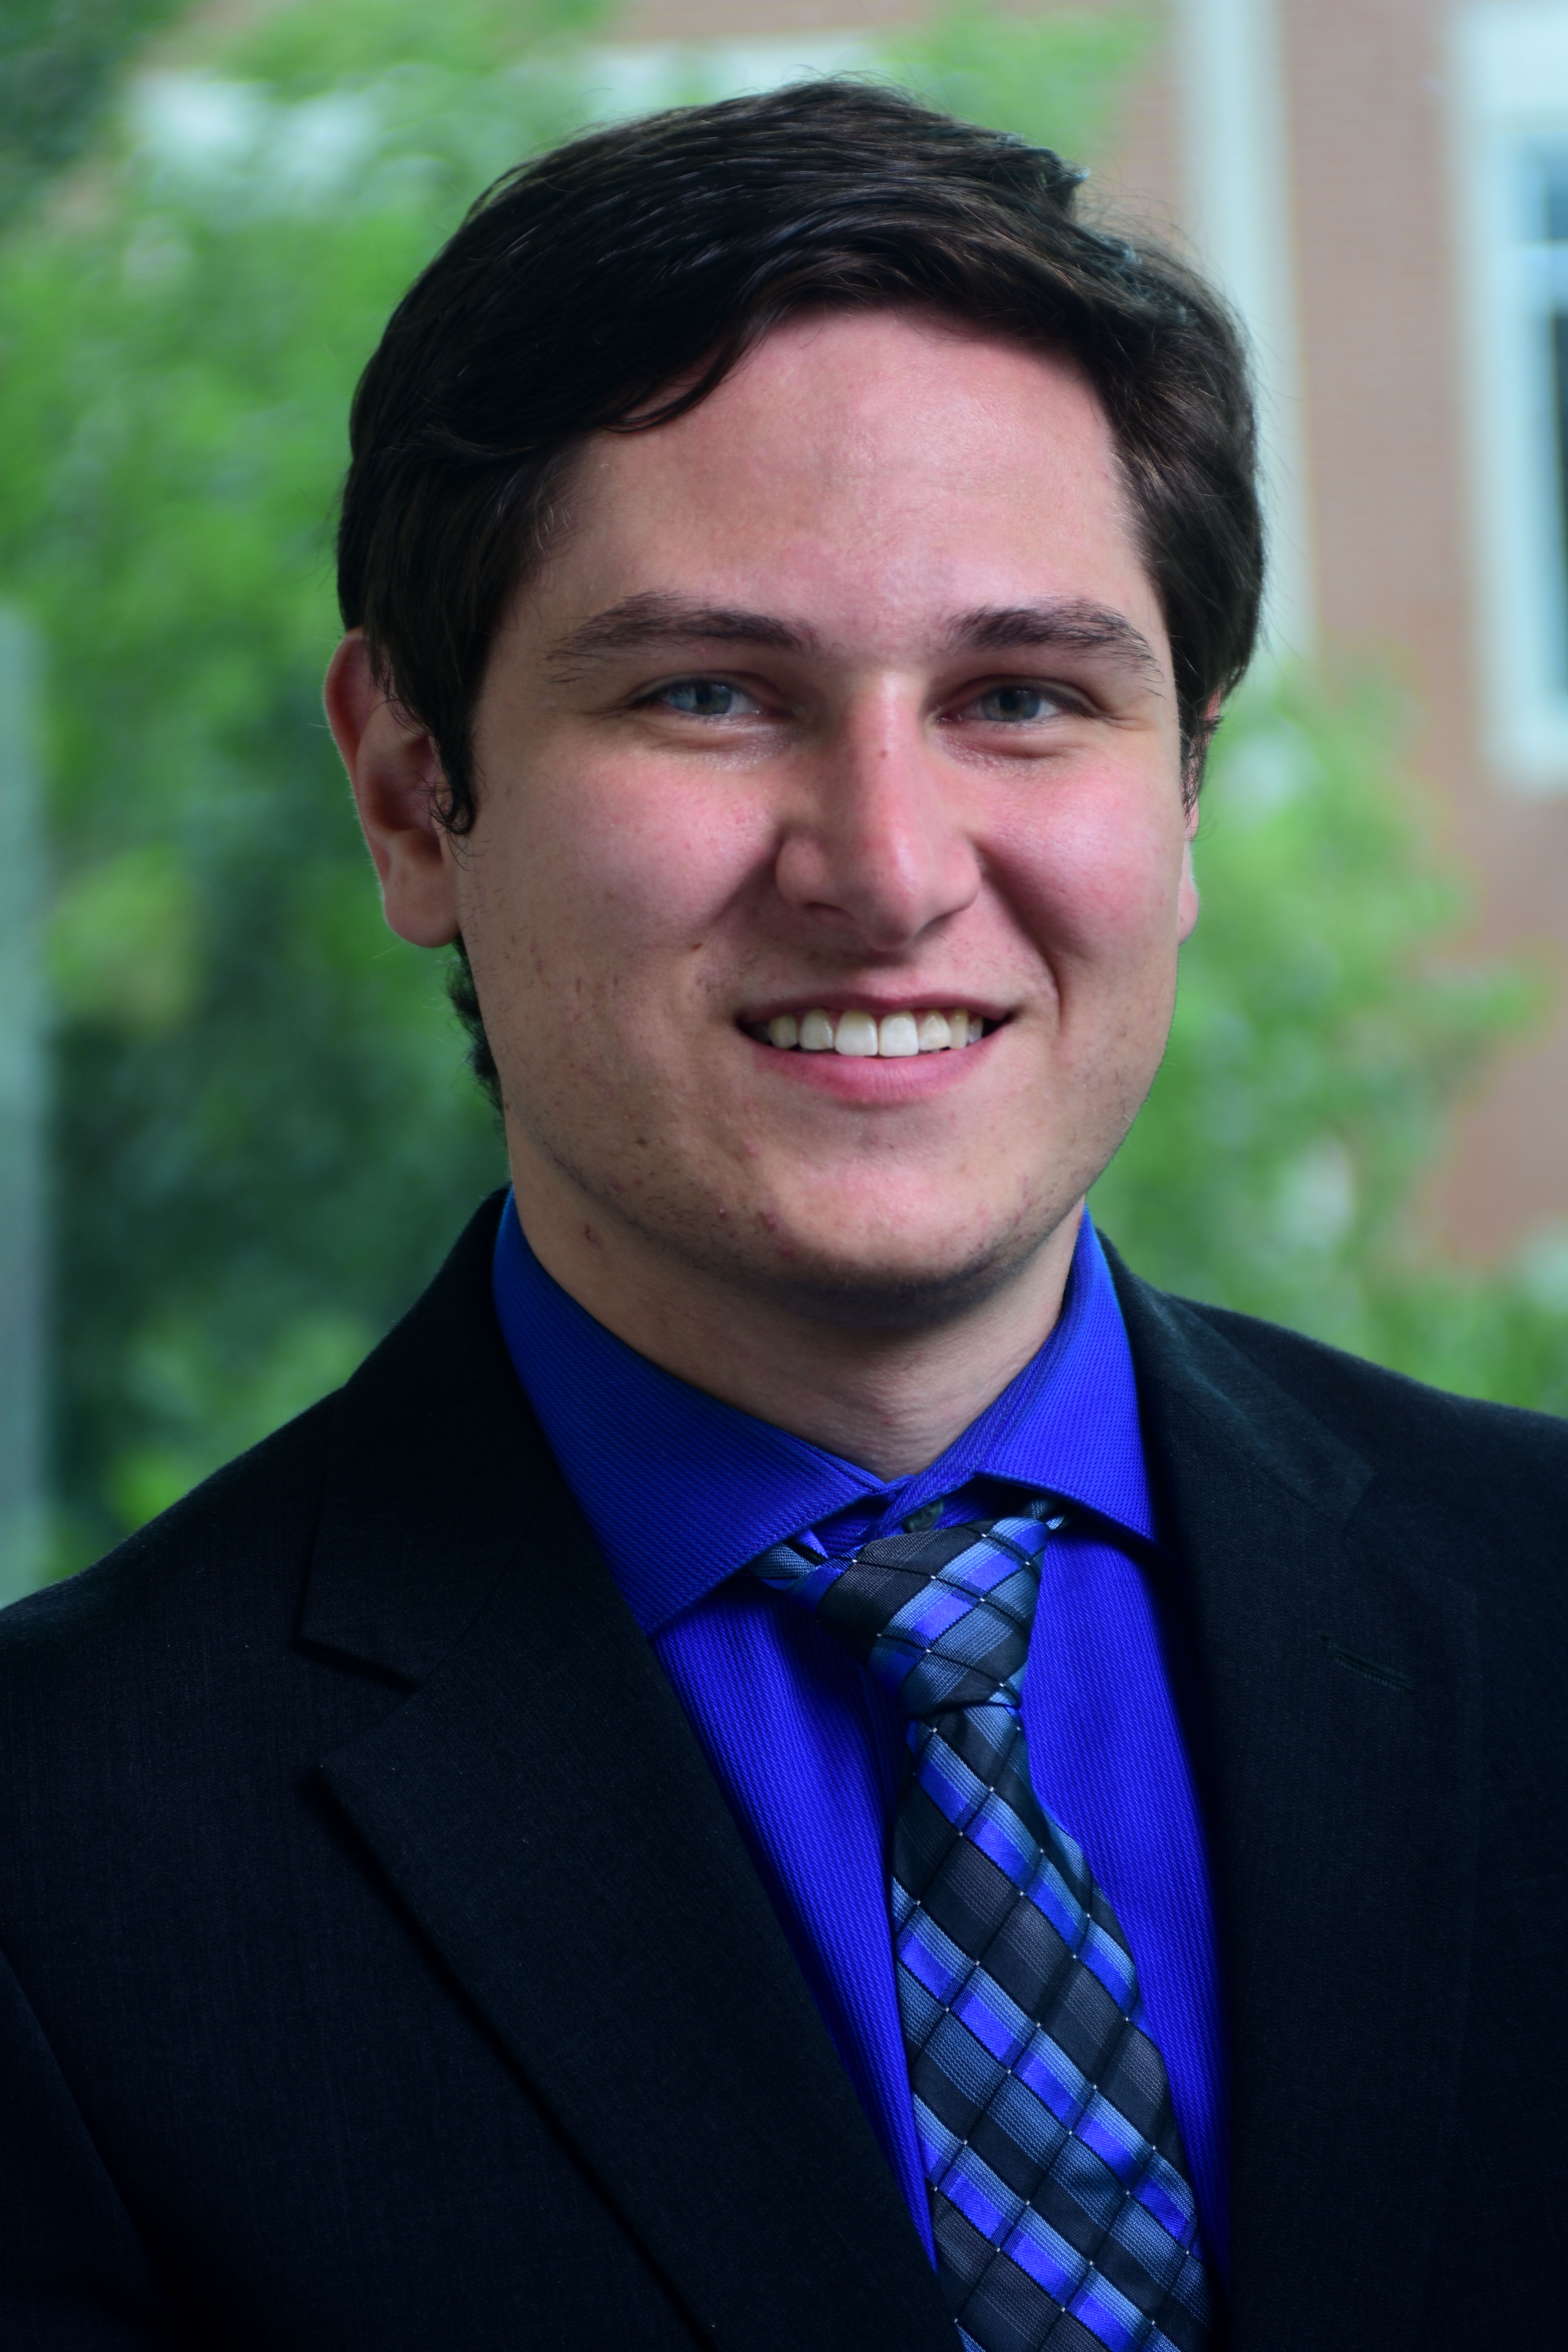
\includegraphics[height=15\baselineskip]{mettlerj.jpg}
	\end{center}
\end{wrapfigure}
$\textbf{Technical Co-Chair - Jeremy Mettler}$\\
Jeremy graduated with a B.S. in Nuclear, Plasma, and Radiological Engineering from UIUC in 2018, and is now attending as a 2nd-year graduate student studying plasma science under Dr. David Ruzic. He has been heavily involved in the UIUC student chapter of ANS since his freshman year, serving on the executive board for three years as External Vice President and President. Jeremy has attended the past five ANS Student Conferences, which serve as an inspiration for his involvement in this proposal process. He is dedicated to making sure that future generations of students are able to have the same amazing experiences through ANS as he had, especially at the ANS Student Conference. Outside of ANS, he has held a summer internship at Oak Ridge National Lab, and is currently focusing his research towards combined laser-plasma systems for materials processing.\\


$\textbf{Financial Co-Chair}$\\\\

$\textbf{Account Coordinator}$\\
$\textbf{Registration Coordinator}$\\
$\textbf{Sponsorship Coordinator}$\\

$\textbf{Technical Subcommittee}$\\\\

$\textbf{Technical Subcommittee Chair}$\\
$\textbf{Sessions Coordinator}$\\
$\textbf{Workshops Coordinator}$\\
$\textbf{Career Fair Coordinator}$\\


$\textbf{Non-Technical Subcommittee}$\\\\

$\textbf{Logistics Chair}$\\
$\textbf{Hotels and Transportation Coordinator}$\\
$\textbf{Hospitality and Catering Coordinator}$\\
$\textbf{Tours Coordinator}$\\
$\textbf{Program Coordinator}$\\



$\textbf{Media Coordinator}$\\



[All committee members must plan on attending the upcoming student conference!]


\subsection{Conflict Resolution}

Committee members should hold professionalism at the forefront of their composure in order to avoid and resolve issues amicably without the involvement of higher powers. As such, members are encouraged to settle conflicts without invoking this protocol. If an issue arises that immediately presents itself as overwhelming, the scope of the issue exceeds an individual’s ability to handle it, or the issue imposes certain implications that jeopardizes the mission of the planning committee, members should not hesitate to refer to this section. In the event of a conflict between members of the planning committee, a document for decision-making and
conflict resolution has been drafted and approved by the general committee. All General Committee members
are expected to abide by the resolution. Key points of the resolution are as follows:
\begin{enumerate}
	\item Subcommittees are encouraged to resolve conflicts internally and as democratically as possible. If an independent resolution cannot be reached, the Co-Chairs should be involved. The Co-Chairs have the final word on all decisions. If the Co-Chairs are unable to agree on a solution, the faculty advisor will be involved.
	\item Conflicts between individual committee members are to be resolved outside of the committee. Should such a conflict jeopradize the mission of the conference the Co-Chairs will be involved. 
	\item Any cases of misconduct or negligence will be handled appropriately by the Co-Chairs.
	\item For extreme cases of misconduct or negligence, separate steps for the removal and replacement of a
	member are outlined for general members, Subcommittee Chairs, and Co-Chairs. These include
	a discussion with the offending member, consultation of the Faculty Advisor, and a hearing with the
	General Committee to decide if removal is necessary.
\end{enumerate}

\subsection{Staffing Requirements}
Staffing for room breakdowns and setups, registration, socials, workshops, tours, etc.  will be supplied by either UIUC ANS members or students of the NPRE department. While it is likely that members of our student chapter will voluntarily fill all the staffing requirements of conference hosted events. If not, we will rely on other student organizations for support including, but not limited to: ACDIS and WIE. Participating in conference events on a staff level is a beneficial experience for any undergraduate who wants to become more familiar with ANS or support their ANS Chapter. Throughout the conference, interacting with registering students, driving groups to tour a scientific facility, and turning rooms for technical sessions provide plentiful opportunities for volunteers to interact with myriad members on a number of levels. Thus, it will be an overall positive experience for the volunteers. Quantitative needs are outlined in Appendix G.

% ===============================================
% Milestones
% ===============================================
\subsection{Milestones}

\begin{center}
\begin{longtable}{c |  c  c}
\hline\hline
Deadline & Task & Responsibility\\
\hline\hline

&November&\\
\hline\hline
& Announcement of 2021 Conference & \\
& Update milestones with lessons learned &\\
& Notify department of selection & Co-Chairs\\
& Confirm Conference Committee & Co-Chairs\\
& Finalize Conference Date & Co-Chairs\\
& Confirm Conference Reservations & Non-Technical\\
& Contact ANS National for support with hotel negotiations& Co-Chairs and Non-Technical\\
& Set up banking through Busey Bank and ANS National& Financial\\
\hline\hline
&December&\\
\hline\hline
&Finalize Facilities Reservations& Non-Technical\\
&Finalize Logo Design& Communications\\
&Begin Designing Website and Social Media& Communications\\
\hline\hline
&$\textbf{2020}$&\\
\hline\hline
&January&\\
\hline\hline
& Finalize meeting schedule& Co-Chairs\\
&&\\
\hline\hline
&February&\\
\hline\hline
& Launch social media plan& Communications\\
& Finalize list of potential speakers& Non-Technical\\
& Finalize technical topics& Technical\\
\hline\hline
&March&\\
\hline\hline
& Contact Speakers and Presenters& Non-Technical and Technical\\
\hline\hline
&April&\\
\hline\hline
& Attend Student Conference at NC State& All\\
& Request lessons learned from NC State& Co-Chairs\\
& Create sponsor letters and contact & General Co-Chair\\
& Prepare tour opportunities& Non-Technical\\
\hline\hline
&May&\\
\hline\hline
& Confirm tours and costs& Non-Technical\\
& Submit Progress Report to SSC& \\
& Create a Call for Papers & Technical and Communications\\
\hline\hline
&June&\\
\hline\hline
& Send Delegates to National Conference& Co-Chairs, All\\
\hline\hline
&July&\\
\hline\hline
& Confirm with all speakers and presenters& \\
& Report on sponsorship& Financial\\
& Reassess budget& Financial\\
\hline\hline
&August&\\
\hline\hline
& Update with sponsors& Financial\\
& Submit second progress to SSC& Co-Chairs\\
\hline\hline
&September&\\
\hline\hline
& Updates on conference deadlines& Financial\\
& Order gift bags& Non-Technical\\
\hline\hline
&October&\\
\hline\hline
& Confirm hotel blocks and contracts& Non-Technical\\
& Registration Opens& Financial\\
& Create and test online paper submission& Technical\\
\hline\hline
&November&\\
\hline\hline
& Attend Winter Conference 2020& Co-Chairs, All\\
& Finalize marketing material& Communications\\
& Report from winter conference & Co-Chairs\\
\hline\hline
&December&\\
\hline\hline
& Update website & Communications \\
& Third progress report to SSC& Co-Chairs\\
& Send out call for papers& Communications\\
\hline\hline
&$\textbf{2021}$&\\
\hline\hline
&January&\\
\hline\hline
& Confirm all judges, panelists, and speakers& Technical\\
& First paper deadline -- send to reviewers & Technical\\
& Recruit student volunteers& All\\
& Finalize tours& Non-Technical\\
& Finalize conference transportation& Non-Technical\\
\hline\hline
&February&\\
\hline\hline
& Finalize program& Communications\\
& Order gift bag items & Financial and Non-Technical\\
& Final Paper Deadline& Technical\\
& Finalize App& Communications\\
& Finalize budget& Financial\\
& Extended Paper Deadline& \\
\hline\hline
&March&\\
\hline\hline
& Print Programs& Communications\\
& Finalize Awards& Technical\\
& Finalize Staff Schedule& Non-Technical\\
& Prepare gift bags, print tags, and banners& Non-Technical\\
& Final progress report to SSC& Co-Chairs\\
\hline\hline
&April&\\
\hline\hline
& Host ANS Student Conference 2021 & \\
& Return seed money& Financial\\
& Process Student Reimbursements& Financial\\
& Finalize financial report& Financial\\
& Submit conference report& Co-Chairs\\
\hline\hline
\end{longtable}
\end{center}